\documentclass[12pt,a4paper,ngerman]{report}
\usepackage{graphicx}
\usepackage{ifpdf}
\ifpdf
   % put here packages only for the PDF:
   \DeclareGraphicsExtensions{.pdf,.png,.jpg,.mps}
   \usepackage{hyperref}
\else
   % put here packages only for the DVI:
\fi

% put all the other packages here:
\usepackage{amsmath}
\usepackage{amsthm}
\usepackage{algorithm}
\usepackage{varwidth}
\usepackage[noend]{algpseudocode}
\usepackage{tikz}
\usetikzlibrary{shapes,shapes.geometric,arrows,fit,calc,positioning,automata}

\newtheorem{theorem}{Satz}
\newtheorem{bem}{Bemerkung}

\usepackage{style}
\algblockdefx[Foreach]{Foreach}{EndForeach}[1]{\textbf{foreach} #1 \textbf{do}}{\textbf{end foreach}}
\begin{document}




\maketitle

\chapter*{Vorwort}
Diese Ausarbeitung entstand im Rahmen eines Studienprojektes im Wahlpflichtmoduls
„Graphentheorie und Graphenalgorithmen“ an der Hochschule RheinMain.


% if we want to shorten the toc
% \setcounter{tocdepth}{0}
\tableofcontents
\listoffigures
\listoftables



\section{Einführung}
\subsection{„Asymmetrisches Traveling Salesman“ Problem}
Das Problem des Handlungsreisenden ist ein
\textbf{NP-hartes} kombinatorisches Problem, bei dem versucht wird in
einem vollständigen gerichtetem Graphen die kürzeste Rundreise zu finden. Jeder
Knoten darf dabei nur einmal besucht werden. Der Zusatz „asymmetrisch“
bedeutet, dass eine Kante zwischen $v_n$ und $v_m$ ein anderes Gewicht
hat als die Kante zwischen $v_m$ und $v_n$.

\subsection{Komplexität}
\begin{theorem}
Die Komplexität zum Herausfinden der kürzesten Rundreise in einem
vollständigen Graphen ist $\mathcal{O}(n!)$. 
\end{theorem}

\begin{proof}
Sei $G=(V,E)$, wobei $V = \{ v_0, v_1, \dotsc, v_n\}$, $E= ?$ ein
vollständiger gerichteter Graph, das bedeutet, von einem
beliebigen Knoten $v_j$ mit $j \leq n$ sind alle anderen Knoten $v_0, v_1, \dotsc, v_n$
erreichbar. Wir starten eine beliebige Rundreise bei dem Knoten $v_j$.
Da wir $v_j$ nicht mehr besuchen dürfen, bleiben uns noch 
$n-1$ Knoten zur Auswahl, die wir von $v_j$ besuchen können. Für den
darauffolgende Knoten bleiben uns $n-2$ Knoten, und so weiter. Dies bedeutet, dass 
die Anzahl der möglichen Touren $(n-1)!$ beträgt.
\begin{align*}
  (n-1)! = (n-1) \cdot (n-2) \cdot \dotsc \cdot 2 \cdot 1
\end{align*}
Da $\mathcal{O}((n-1)!) \in \mathcal{O}(n!)$ gilt, war die Annahme
korrekt.
\end{proof}
\begin{bem}
Die Anzahl der Möglichen Rundreisen bei einer Knotenanzahl von $4$ wären also
$(4-1)! = 1 \cdot 2 \cdot 3 =\underline{\underline{6}}$. Wählen wir $n = 20$ würde die
Anzahl der möglichen Rundreisen bereits $(20-1)! =
\underline{\underline{121645100408832000}}$ betragen.
Das Problem ist daher vermutlich nicht in polynomieller Zeit lösbar.
\end{bem}

\subsection{Lösungsidee}
In der Praxis werden heutzutage trotz allem „gute“ Lösungen benötigt.
Eine direkte Berechnung der besten Lösung ist aber für eine große
Knotenanzahl nicht praxistauglich. In dieser Ausarbeitung wird
vorgestellt, wie man gute Lösungen mit einem sogenannten „evolutionären
Algorithmus“ heuristisch findet.

\chapter{Generalized Asymmetric Partition Crossover}

\label{gapx_einleitung}
\section{Einleitung}
Der „Generalized Asymmetric Partition Crossover“ (GAPX) ist ein
Rekombinationsoperator, der als Teil eines evolutionären Algorithmus
verwendet werden kann~\cite{gapx}. Aufgabe einer Rekombination (auch
Crossover genannt) beim ATSP ist es aus
zwei gegebenen Rundreisen $G_1$, $G_2$ ein Kind (auch Offspring genannt)
$G_o$ zu erzeugen.


\begin{algorithm}
\caption{Crossover in einem EA}\label{alg:crossover_ea}
\begin{algorithmic}[1]
\Procedure{Crossover}{$G_1,G_2$}\Comment{}
\State $G_o\gets gapx(G_1,G_2)$\Comment{In 2.2 beschrieben}
\State \textbf{return} $G_o$
\EndProcedure
\end{algorithmic}
\end{algorithm}
\noindent
GAPX versucht durch ein bestimmtes Verfahren die beiden Rundreisen zu
partitionieren und anhand der kürzesten Wege innerhalb der Komponenten
das neue Kind $G_o$ zu erzeugen. Die
Funktionsweise, die im nachfolgenden Kapitel beschrieben wird, basiert
auf~\cite{gapx}.


\section{Funktionsweise}
Seien $G_1$ und $G_2$ beliebige Rundreisen, beide erzeugt aus einem
vollständigen Graphen $G$. Zunächst werden $G_1$ und $G_2$ in einem
gemeinsamen Graphen $G_u$ zusammengeführt.
\newpage
%% Bild mergen von G1, G2
\begin{figure}[hb]
\centering
\renewcommand{\arraystretch}{3.5}
\begin{tabular}{ c c c }
$G_1$ & $G_2$ & $G_u$ \\
\resizebox{90pt}{90pt}{

  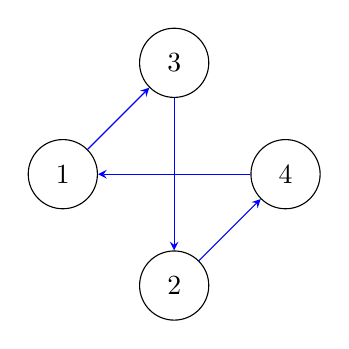
\begin{tikzpicture}[%
    >=stealth,
    node distance=2cm,
    on grid,
    auto
  ]
  \node[state] (1){1};
  \node[state] (3) [above right of=1]{3};
  \node[state] (2) [below right of=1]{2};
  \node[state] (4) [below right of=3]{4};
  
  \path[->] (1) edge [blue, bend left=0] node  {} (3);
  \path[->] (3) edge [blue, bend left=0] node  {} (2);
  \path[->] (2) edge [blue, bend left=0] node  {} (4);
  \path[->] (4) edge [blue, bend left=0] node  {} (1);
  
  \end{tikzpicture}
} 

& 

\resizebox{90pt}{90pt}{

  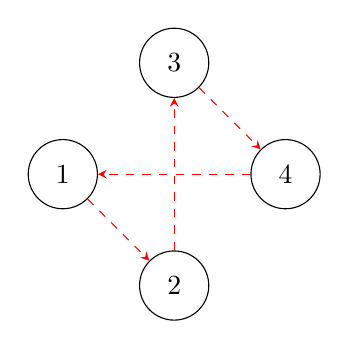
\begin{tikzpicture}[%
    >=stealth,
    node distance=2cm,
    on grid,
    auto
  ]
  \node[state] (1){1};
  \node[state] (3) [above right of=1]{3};
  \node[state] (2) [below right of=1]{2};
  \node[state] (4) [below right of=3]{4};

  \path[->] (1) edge [red, dashed, left=0] node  {} (2);
  \path[->] (2) edge [red, dashed, left=0] node  {} (3);
  \path[->] (3) edge [red, dashed, left=0] node  {} (4);
  \path[->] (4) edge [red, dashed, left=0] node  {} (1);

  \end{tikzpicture}
} 

&

\resizebox{90pt}{90pt}{

  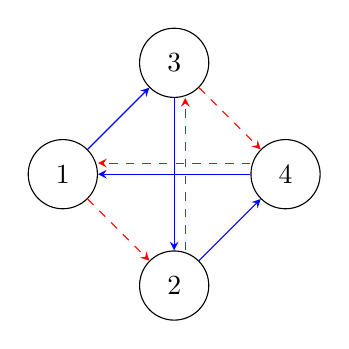
\begin{tikzpicture}[%
    >=stealth,
    node distance=2cm,
    on grid,
    auto
  ]
  \node[state] (1){1};
  \node[state] (3) [above right of=1]{3};
  \node[state] (2) [below right of=1]{2};
  \node[state] (4) [below right of=3]{4};

  \path[->] (1) edge [blue, bend left=0] node  {} (3);
  \path[->] (3) edge [blue, bend left=0] node  {} (2);
  \path[->] (2) edge [blue, bend left=0] node  {} (4);
  \path[->] (4) edge [blue, bend left=0] node  {} (1);

  \path[->] (1) edge [red, dashed, left=0] node  {} (2);
  \path[->] ([xshift=0.4em] 2.north) edge 
      [red, dashed, left=0] node  {} ([xshift=0.4em] 3.south);
  \path[->] (3) edge [red, dashed, left=0] node  {} (4);
  \path[->] ([yshift=0.4em] 4.west) edge 
      [red, dashed, left=0] node  {} ([yshift=0.4em] 1.east);

  \end{tikzpicture}
} 
\end{tabular}
\renewcommand{\arraystretch}{1}
\caption[Beispiel einer Zusammenlegung von Graphen]{
Beispiel für das Zusammenführen der Graphen $G_1$ und $G_2$ zu
dem neuen Graphen $G_u$ anhand zwei Rundreisen mit je vier Knoten.
}
\end{figure}
%%\begin{bem}
%%  Streng genommen ist $G_u$ ein Multigraph, da doppelte Kanten zwischen
%%  Knoten existieren können, jedoch hat dies die Implementierung nicht
%%  eingeschränkt, da ein „normaler Graph“ eine Spezielform eines
%%  Multigraphen ist.
%%\end{bem}
\noindent
Nachfolgend betrachten wir zur Erklärung zwei Graphen $G_1$ und $G_2$ mit elf Knoten. 
Nach der Zusammenführung der beiden Graphen in $G_u$ muss für jeden 
Knoten $v$ aus $G_u$, der \textit{vier} Nachbarn hat, ein
sogenannter Ghost-Knoten $v'$ nach $v$ eingefügt werden. Durch das
Einführen der zusätzlichen Knoten ist es möglich mehr Komponenten im
Graphen zu finden. Zusätzlich muss eine
Kante mit dem Gewicht $0$ zwischen $v$ und $v'$ eingefügt werden. 
Der Graph $G_u$ mit eingefügten Ghost-Knoten an den entsprechenden Stellen kennzeichnen wir als $G_u'$.
\begin{figure}[hb]
\label{fig:ghostnodes}
\centering
\begin{tabular}{ c c }
\resizebox{120pt}{170pt}{
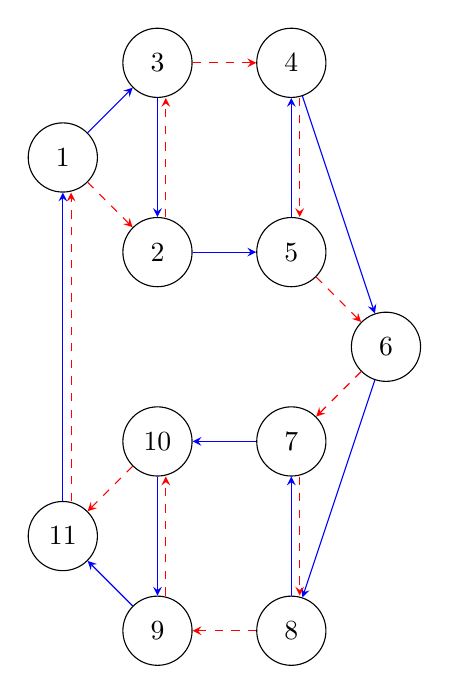
\begin{tikzpicture}[%
>=stealth,
node distance=1.7cm,
on grid
]
\node[state] (1)              {1};


\node[state] (3) [above right of=1]             {3};
\node[state] (2) [below right of=1]            {2};
\node[state] (4) [right of=3]             {4};
\node[state] (5) [right of=2]             {5};

\node[state] (6) [below right of=5] {6};

\node[state] (7) [below left of=6] {7};
\node[state] (10) [left of=7] {10};

\node[state] (11) [below left of=10] {11};

\node[state] (9) [below right of=11] {9};
\node[state] (8) [right of=9] {8};

% solid: parent 1
\path[->] (1) edge [blue, bend left=0] node  {} (3);
\path[->] (3) edge [blue, bend left=0] node  {} (2);
\path[->] (2) edge [blue, bend left=0] node  {} (5);
\path[->] (5) edge [blue, bend left=0] node  {} (4);
\path[->] (4) edge [blue, bend left=0] node  {} (6);
\path[->] (6) edge [blue, bend left=0] node  {} (8);
\path[->] (8) edge [blue, bend left=0] node  {} (7);
\path[->] (7) edge [blue, bend left=0] node  {} (10);
\path[->] (10) edge [blue, bend left=0] node  {} (9);
\path[->] (9) edge [blue, bend left=0] node  {} (11);
\path[->] (11) edge [blue, bend left=0] node  {} (1);

% dashed: parent 2
\path[->] (1) edge [bend left=0, dashed, red] node {} (2);
\path[->] ([xshift=0.7ex] 2.north) edge [red, dashed] node {}
         ([xshift=0.7ex] 3.south);
\path[->] (3) edge [red, dashed] node {}
         (4);
\path[->] ([xshift=0.7ex] 4.south) edge [red, dashed] node {}
         ([xshift=0.7ex] 5.north);
\path[->] (5) edge [red, dashed] node {}
         (6);
\path[->] (6) edge [red, dashed] node {}
         (7);
\path[->] ([xshift=0.7ex] 7.south) edge [red, dashed] node {}
         ([xshift=0.7ex] 8.north);
\path[->] (8) edge [red, dashed] node {}
         (9);
\path[->] ([xshift=0.7ex] 9.north) edge [red, dashed] node {}
         ([xshift=0.7ex] 10.south);
\path[->] (10) edge [red, dashed] node {}
         (11);
\path[->] ([xshift=0.7ex] 11.north) edge [red, dashed] node {}
         ([xshift=0.7ex] 1.south);
\end{tikzpicture}
}

&
\resizebox{120pt}{170pt}{
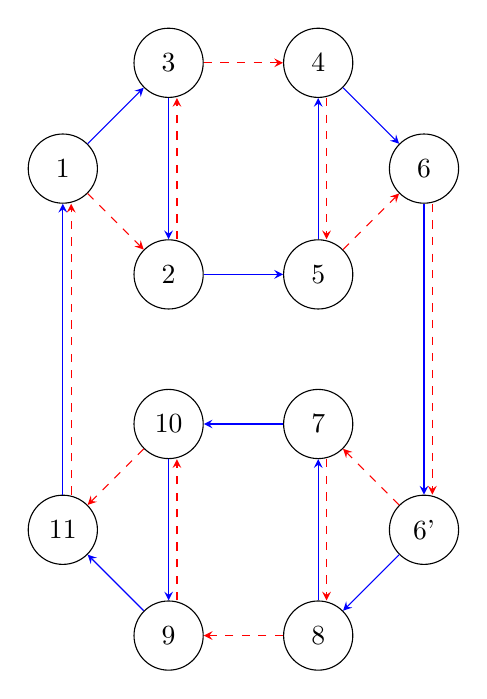
\begin{tikzpicture}[%
>=stealth,
node distance=1.9cm,
on grid,
auto
]
\node[state] (1){1};
\node[state] (3) [above right of=1]{3};
\node[state] (2) [below right of=1]{2};
\node[state] (4) [right of=3]{4};
\node[state] (5) [right of=2]{5};
\node[state] (6) [above right of=5] {6};
\node[state] (7) [below of=5] {7};
\node[state] (6') [below right of=7] {6'};
\node[state] (10) [left of=7] {10};
\node[state] (11) [below left of=10] {11};
\node[state] (9) [below right of=11] {9};
\node[state] (8) [right of=9] {8};

% solid: parent 1
\path[->] (1) edge [blue, bend left=0] node  {} (3);
\path[->] (3) edge [blue, bend left=0] node  {} (2);
\path[->] (2) edge [blue, bend left=0] node  {} (5);
\path[->] (5) edge [blue, bend left=0] node  {} (4);
\path[->] (6') edge [blue, bend left=0] node  {} (8);
\path[->] (4) edge [blue, bend left=0] node  {} (6);
\path[->] (8) edge [blue, bend left=0] node  {} (7);
\path[->] (7) edge [blue, bend left=0] node  {} (10);
\path[->] (10) edge [blue, bend left=0] node  {} (9);
\path[->] (9) edge [blue, bend left=0] node  {} (11);
\path[->] (11) edge [blue, bend left=0] node  {} (1);
\path[->] (6) edge [blue, bend left=0] node  {} (6');

% dashed: parent 2
\path[->] (1) edge [bend left=0, dashed, red] node {} (2);
\path[->] ([xshift=0.7ex] 2.north) edge [red, dashed] node {}
         ([xshift=0.7ex] 3.south);
\path[->] (3) edge [red, dashed] node {}
         (4);
\path[->] ([xshift=0.7ex] 4.south) edge [red, dashed] node {}
         ([xshift=0.7ex] 5.north);
\path[->] (5) edge [red, dashed] node {}
         (6);
\path[->] (6') edge [red, dashed] node {}
         (7);
\path[->] ([xshift=0.7ex] 7.south) edge [red, dashed] node {}
         ([xshift=0.7ex] 8.north);
\path[->] (8) edge [red, dashed] node {}
         (9);
\path[->] ([xshift=0.7ex] 9.north) edge [red, dashed] node {}
         ([xshift=0.7ex] 10.south);
\path[->] (10) edge [red, dashed] node {}
         (11);
\path[->] ([xshift=0.7ex] 11.north) edge [red, dashed] node {}
         ([xshift=0.7ex] 1.south);
  \path[->] ([xshift=0.7ex] 6.south) edge [red, dashed] node {}
         ([xshift=0.7ex] 6'.north);

\end{tikzpicture}
}
\end{tabular}
\caption[Beispiel Einfügung von Ghost-Knoten]{Links: Ein Graph $G_u$ vor der Einführung von
Ghostknoten. Rechts: Der Graph $G_u'$ mit dem eingefügten Ghostknoten $6'$.
Blaue Linie: $G_1$, erstes Elternteil; rote, gestrichelte Linie: $G_2$,
zweites Elternteil}
\end{figure}
\newpage
\noindent
Nachdem alle Ghost-Knoten eingefügt wurden, müssen genau jene Kanten entfernt
werden, die in $G_1$ \textbf{und} $G_2$ vorkommen, um eine
Partitionierung des Graphen vorzunehmen. Zusätzlich
müssen die Kanten entfernt werden, die bei der Generierung der
Ghost-Knoten neu eingefügt wurden. In \hyperref[fig:ghostnodes]{Abbildung 2.2} wäre dies die Kante
zwischen $6$ und $6'$. Die Menge dieser entfernten Kanten nennen wir
nachfolgend $E_c$ und werden auch „Common-Edges“ genannt. Die Menge
$E_c$
beinhaltet also genau die Kanten, die in beiden Elternteilen vorkommen. Die
Menge $E_c$ wird nun in die Kantenmenge von $G_o$ (dem Offspring)
eingefügt.
\begin{figure}[hb]
  \label{fig:offspring_1}
\centering
\resizebox{100pt}{140pt}{
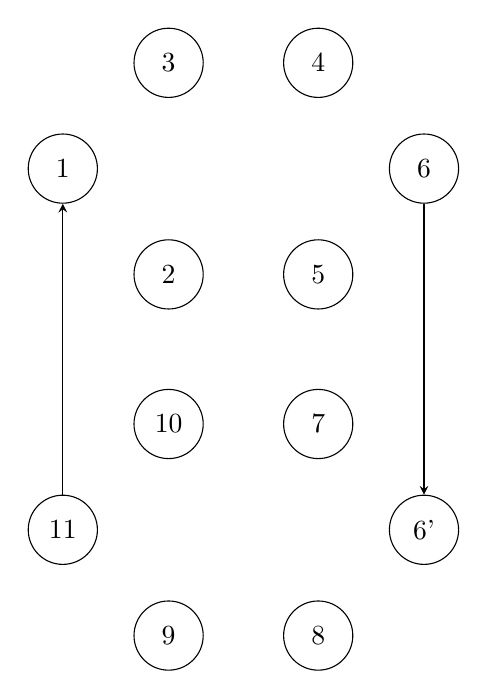
\begin{tikzpicture}[%
>=stealth,
node distance=1.9cm,
on grid,
auto
]
\node[state] (1){1};
\node[state] (3) [above right of=1]{3};
\node[state] (2) [below right of=1]{2};
\node[state] (4) [right of=3]{4};
\node[state] (5) [right of=2]{5};
\node[state] (6) [above right of=5] {6};
\node[state] (7) [below of=5] {7};
\node[state] (6') [below right of=7] {6'};
\node[state] (10) [left of=7] {10};
\node[state] (11) [below left of=10] {11};
\node[state] (9) [below right of=11] {9};
\node[state] (8) [right of=9] {8};

% solid: parent 1
\path[->] (11) edge [bend left=0] node  {} (1);
\path[->] (6) edge [bend left=0] node  {} (6');

\end{tikzpicture}
}
  \caption[Kind $G_o$ nach Einfügen der gemeinsamen Kantenmenge $E_c$]
  {Das Kind $G_o$ im momentanen Zustand. In
  \hyperref[fig:ghostnodes]{Abbildung 2.2} sind Ghost-Knoten eingefügt
  worden. $E_c = \{(6,6'),(1,11)\}$. Die Kante $(6,6')$ ist durch das
  Einfügen eines Ghost-Knoten entstanden. Die Kante $(1,11)$ ist in beiden
  Rundreisen $G_1$ und $G_2$ vorhanden. $E_c$ wurde in $G_o$ eingefügt.}
\end{figure}
\noindent
Durch das Entfernen von $E_c$ in $G_u'$ haben wir eine Partitionierung
des Graphen erreicht. Der Graph $G_u'$ wurde in seine Komponenten
zerlegt. Es sollen nun „gute“ Wege durch die Komponenten gefunden
werden.
\begin{figure}[H]
  \label{fig:components}
\centering
  \begin{tabular}{c c}
\resizebox{120pt}{170pt}{
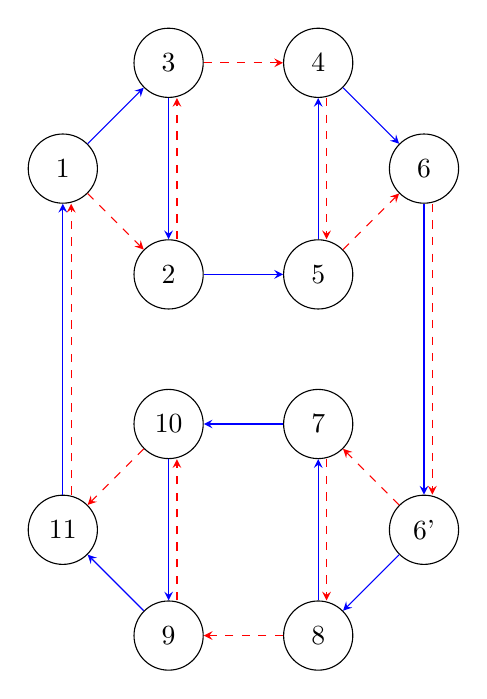
\begin{tikzpicture}[%
>=stealth,
node distance=1.9cm,
on grid,
auto
]
\node[state] (1){1};
\node[state] (3) [above right of=1]{3};
\node[state] (2) [below right of=1]{2};
\node[state] (4) [right of=3]{4};
\node[state] (5) [right of=2]{5};
\node[state] (6) [above right of=5] {6};
\node[state] (7) [below of=5] {7};
\node[state] (6') [below right of=7] {6'};
\node[state] (10) [left of=7] {10};
\node[state] (11) [below left of=10] {11};
\node[state] (9) [below right of=11] {9};
\node[state] (8) [right of=9] {8};

% solid: parent 1
\path[->] (1) edge [blue, bend left=0] node  {} (3);
\path[->] (3) edge [blue, bend left=0] node  {} (2);
\path[->] (2) edge [blue, bend left=0] node  {} (5);
\path[->] (5) edge [blue, bend left=0] node  {} (4);
\path[->] (6') edge [blue, bend left=0] node  {} (8);
\path[->] (4) edge [blue, bend left=0] node  {} (6);
\path[->] (8) edge [blue, bend left=0] node  {} (7);
\path[->] (7) edge [blue, bend left=0] node  {} (10);
\path[->] (10) edge [blue, bend left=0] node  {} (9);
\path[->] (9) edge [blue, bend left=0] node  {} (11);
\path[->] (11) edge [blue, bend left=0] node  {} (1);
\path[->] (6) edge [blue, bend left=0] node  {} (6');

% dashed: parent 2
\path[->] (1) edge [bend left=0, dashed, red] node {} (2);
\path[->] ([xshift=0.7ex] 2.north) edge [red, dashed] node {}
         ([xshift=0.7ex] 3.south);
\path[->] (3) edge [red, dashed] node {}
         (4);
\path[->] ([xshift=0.7ex] 4.south) edge [red, dashed] node {}
         ([xshift=0.7ex] 5.north);
\path[->] (5) edge [red, dashed] node {}
         (6);
\path[->] (6') edge [red, dashed] node {}
         (7);
\path[->] ([xshift=0.7ex] 7.south) edge [red, dashed] node {}
         ([xshift=0.7ex] 8.north);
\path[->] (8) edge [red, dashed] node {}
         (9);
\path[->] ([xshift=0.7ex] 9.north) edge [red, dashed] node {}
         ([xshift=0.7ex] 10.south);
\path[->] (10) edge [red, dashed] node {}
         (11);
\path[->] ([xshift=0.7ex] 11.north) edge [red, dashed] node {}
         ([xshift=0.7ex] 1.south);
  \path[->] ([xshift=0.7ex] 6.south) edge [red, dashed] node {}
         ([xshift=0.7ex] 6'.north);

\end{tikzpicture}
}
&
\resizebox{120pt}{170pt}{
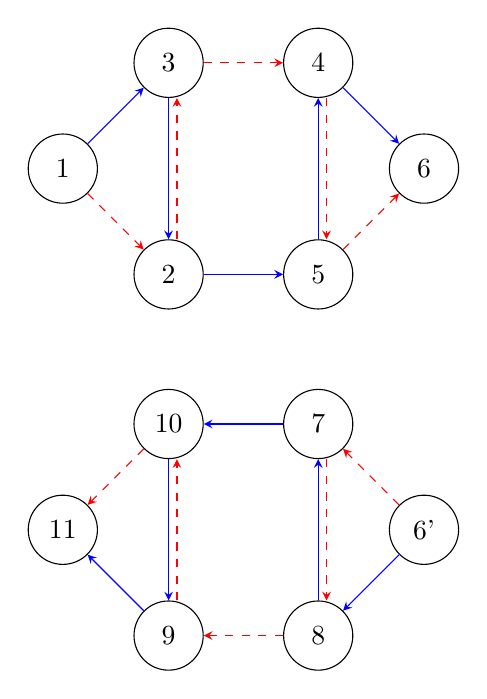
\begin{tikzpicture}[%
>=stealth,
node distance=1.9cm,
on grid,
auto
]
\node[state] (1){1};
\node[state] (3) [above right of=1]{3};
\node[state] (2) [below right of=1]{2};
\node[state] (4) [right of=3]{4};
\node[state] (5) [right of=2]{5};
\node[state] (6) [above right of=5] {6};
\node[state] (7) [below of=5] {7};
\node[state] (6') [below right of=7] {6'};
\node[state] (10) [left of=7] {10};
\node[state] (11) [below left of=10] {11};
\node[state] (9) [below right of=11] {9};
\node[state] (8) [right of=9] {8};

% solid: parent 1
\path[->] (1) edge [blue, bend left=0] node  {} (3);
\path[->] (3) edge [blue, bend left=0] node  {} (2);
\path[->] (2) edge [blue, bend left=0] node  {} (5);
\path[->] (5) edge [blue, bend left=0] node  {} (4);
\path[->] (6') edge [blue, bend left=0] node  {} (8);
\path[->] (4) edge [blue, bend left=0] node  {} (6);
\path[->] (8) edge [blue, bend left=0] node  {} (7);
\path[->] (7) edge [blue, bend left=0] node  {} (10);
\path[->] (10) edge [blue, bend left=0] node  {} (9);
\path[->] (9) edge [blue, bend left=0] node  {} (11);

% dashed: parent 2
\path[->] (1) edge [bend left=0, dashed, red] node {} (2);
\path[->] ([xshift=0.7ex] 2.north) edge [red, dashed] node {}
         ([xshift=0.7ex] 3.south);
\path[->] (3) edge [red, dashed] node {}
         (4);
\path[->] ([xshift=0.7ex] 4.south) edge [red, dashed] node {}
         ([xshift=0.7ex] 5.north);
\path[->] (5) edge [red, dashed] node {}
         (6);
\path[->] (6') edge [red, dashed] node {}
         (7);
\path[->] ([xshift=0.7ex] 7.south) edge [red, dashed] node {}
         ([xshift=0.7ex] 8.north);
\path[->] (8) edge [red, dashed] node {}
         (9);
\path[->] ([xshift=0.7ex] 9.north) edge [red, dashed] node {}
         ([xshift=0.7ex] 10.south);
\path[->] (10) edge [red, dashed] node {}
         (11);

\end{tikzpicture}
}

\end{tabular}
\caption[Partitionierung von $G_u'$ nach Löschen von $E_c$]{Rechts oben:
$G_{c_1}$ der Teilgraph mit den Knoten $1,2,3,4,5,6$, 
Rechts unten: $G_{c_2}$ ist der Teilgraph mit den Knoten $11,9,10,7,8,6'$ }
\end{figure}
\noindent
Jede Komponente wird als Teilgraph $G_{c_k}$ gekennzeichnet, wobei $k
\leq $Anzahl der Komponenten in $G_u'$. 
Wir definieren $G_c = \bigcup_{1 \leq k \leq n}{\{G_{c_k}\}}$, wobei $n$ die Anzahl 
der Komponenten in $G_u'$ ist.
Für alle Komponenten in $G_c$ müssen die Menge der Eingangs- und
Ausgangsknoten festgestellt werden. Hierfür werden zwei Funktionen
definiert:
\begin{itemize}
  \item $comp_{in}(G_{c_k}, E_c)$ - ermittelt die Menge der
    Eingangsknoten von $G_{c_k}$ 
  \item $comp_{out}(G_{c_k}, E_c)$ - ermittelt die Menge der
    Ausgangsknoten von $G_{c_k}$ 
\end{itemize}
\begin{algorithm}[H]
  \caption{Ermittlung Eingangsknoten in $G_{c_k}$}\label{alg:comp_in}
\begin{algorithmic}[1]
  \Procedure{$comp_{in}$}{$G_{c_k}, E_c$}
    \State $V \gets vertices(G_{c_k})$
    \State $Entry \gets list()$
    \Foreach{$v \in]V$}
      \State $g = has\_ghostnode\_in\_comp(G_{c_k}, v)$
      \If {$\neg g \land in\_degree(G_{c_k}, v) = 0$}
      \Comment{In-Degree}    
        \State $Entry \gets append(Entry, v)$
      \EndIf
    \EndForeach
    \State \textbf{return} $Entry$
  \EndProcedure
\end{algorithmic}
\end{algorithm}
\begin{algorithm}[H]
\caption{Ermittlung Ausgangsknoten in $G_{c_k}$}\label{alg:comp_out}
\begin{algorithmic}[1]
  \Procedure{$comp_{out}$}{$G_{c_k}, E_c$}
    \State $V \gets vertices(G_{c_k})$
    \State $Exit \gets list()$
    \Foreach{$v \in V$}
      \State $g = has\_ghostnode\_in\_comp(G_{c_k}, v)$
      \If {$\neg g \land out\_degree(G_{c_k}, v) = 0$}
      \Comment{Out-Degree} 
        \State $Exit \gets append(Exit, v)$
      \EndIf
    \EndForeach
    \State \textbf{return} $Exit$
  \EndProcedure
\end{algorithmic}
\end{algorithm}
\noindent
Die prinzipielle Vorgehensweise der beiden Funktionen ist das Prüfen 
der eingehenden beziehungsweise ausgehenden Kanten. Ein Knoten $v$ kommt
nur als Eingangspunkt in Frage, wenn keine eingehenden Kanten für $v$
existieren. Ein ausgehender Knoten kann hingegen keine ausgehenden Kanten
besitzen.
\begin{bem}
  Es können Komponenten existieren welche, nicht nur einen Eingangs- und
  einen Ausgangsknoten haben. Tatsächlich gibt es sehr häufig
  Partitionierungen mit Komponenten, die drei oder vier Eingänge
  beziehungsweise Ausgänge besitzen. Die Algorithmen 3 und 4 beachten
  diesen Umstand.
\end{bem}
\begin{bem}
  Die Funktion $has\_ghostnode\_in\_comp(G_{c_k}, v)$ ist hier nicht
  ausführlich erläutert. Sie überprüft, ob für einen Knoten $v$ ein
  entsprechender Ghost-Knoten $v'$ eingefügt wurde, wobei sich $v$ und
  $v'$ innerhalb der selben Komponente $G_{c_k}$ befinden. Ist dies der Fall, gibt
  die Funktion den Wert true zurück. Knoten, für die ein entsprechender
  Ghost-Knoten innerhalb der Komponente existiert, können nicht als
  Eingangs- oder Ausgangspunkt verwendet werden, da sie die Komponente
  in weitere Teile aufspalten würde.
\end{bem}
\noindent
Mit den Informationen über Eingangs- und Ausgangsknoten ist der „Weg“ 
einer Komponente zum Teil bekannt. Man startet in einem Eingangsknoten und endet
in einem Ausgangsknoten. Der Weg innerhalb der Komponente muss nun
näher untersucht werden.
Für jede Komponente in $G_c$ muss überprüft werden,
ob für beide Elternteile $G_1$, $G_2$ ein Weg vom Eingangsknoten zum
Ausgangsknoten führt. Der Weg muss zudem durch alle Knoten der
Komponente führen. Nur dann ist die Partitionierung gültig. Wenn die
Partitionierung ungültig ist, kann kein Kind erzeugt werden.
Dieser Vorgang ist in \hyperref[fig:entry_exit]{Abbildung 2.5} an einem Beispiel demonstriert.

Als letzter Schritt von GAPX muss für jede Komponente in $G_c$ berechnet werden,
ob der Weg von $G_1$, der vom Eingangsknoten zum Ausgangsknoten führt,
günstiger ist als der von $G_2$. Der kürzere Teilweg, beziehungsweise die
Kanten, die diesen Weg repräsentieren, werden in den Graphen des
Offsprings $G_o$ übernommen. 

\begin{figure}
  \label{fig:entry_exit}
\centering
\begin{tabular}{l|c|c}
 & $G_1$ & $G_2$ \\
\hline
\rule{0pt}{15.5ex}
$G_{c_1}$ &

\resizebox{120pt}{80pt}{
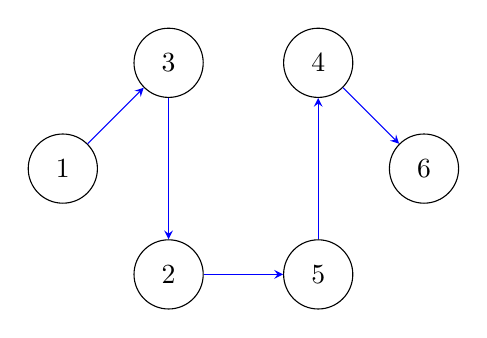
\begin{tikzpicture}[%
>=stealth,
node distance=1.9cm,
on grid,
auto
]
\node[state] (1){1};
\node[state] (3) [above right of=1]{3};
\node[state] (2) [below right of=1]{2};
\node[state] (4) [right of=3]{4};
\node[state] (5) [right of=2]{5};
\node[state] (6) [above right of=5] {6};

% solid: parent 1
\path[->] (1) edge [blue, bend left=0] node  {} (3);
\path[->] (3) edge [blue, bend left=0] node  {} (2);
\path[->] (2) edge [blue, bend left=0] node  {} (5);
\path[->] (5) edge [blue, bend left=0] node  {} (4);
\path[->] (4) edge [blue, bend left=0] node  {} (6);

\end{tikzpicture}
}

  &
\resizebox{120pt}{80pt}{
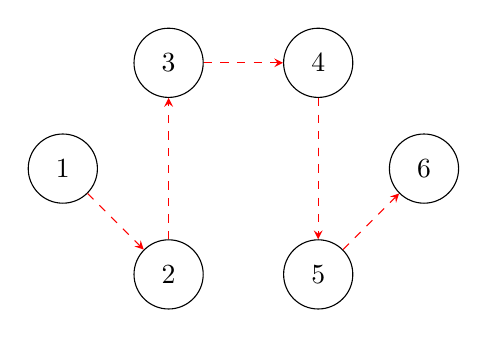
\begin{tikzpicture}[%
>=stealth,
node distance=1.9cm,
on grid,
auto
]
\node[state] (1){1};
\node[state] (3) [above right of=1]{3};
\node[state] (2) [below right of=1]{2};
\node[state] (4) [right of=3]{4};
\node[state] (5) [right of=2]{5};
\node[state] (6) [above right of=5] {6};

% solid: parent 1
\path[->] (1) edge [red, dashed, bend left=0] node  {} (2);
\path[->] (2) edge [red, dashed, bend left=0] node  {} (3);
\path[->] (3) edge [red, dashed, bend left=0] node  {} (4);
\path[->] (4) edge [red, dashed, bend left=0] node  {} (5);
\path[->] (5) edge [red, dashed, bend left=0] node  {} (6);
\end{tikzpicture}
}
\\
\hline
\rule{0pt}{15.5ex}
  $G_{c_2}$ &
\resizebox{120pt}{80pt}{
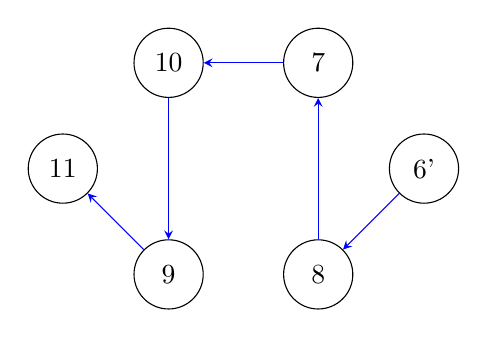
\begin{tikzpicture}[%
>=stealth,
node distance=1.9cm,
on grid,
auto
]
\node[state] (11){11};
\node[state] (10) [above right of=11]{10};
\node[state] (9) [below right of=11]{9};
\node[state] (7) [right of=10]{7};
\node[state] (8) [right of=9]{8};
\node[state] (6') [above right of=8] {6'};

% solid: parent 1
\path[->] (6') edge [blue, bend left=0] node  {} (8);
\path[->] (8) edge [blue, bend left=0] node  {} (7);
\path[->] (7) edge [blue, bend left=0] node  {} (10);
\path[->] (10) edge [blue, bend left=0] node  {} (9);
\path[->] (9) edge [blue, bend left=0] node  {} (11);
\end{tikzpicture}
}
  &
\resizebox{120pt}{80pt}{
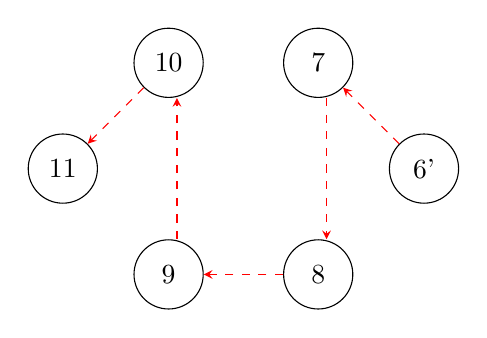
\begin{tikzpicture}[%
>=stealth,
node distance=1.9cm,
on grid,
auto
]
\node[state] (11){11};
\node[state] (10) [above right of=11]{10};
\node[state] (9) [below right of=11]{9};
\node[state] (7) [right of=10]{7};
\node[state] (8) [right of=9]{8};
\node[state] (6') [above right of=8] {6'};

% solid: parent 1
\path[->] (6') edge [red, dashed] node {}
         (7);
\path[->] ([xshift=0.7ex] 7.south) edge [red, dashed] node {}
         ([xshift=0.7ex] 8.north);
\path[->] (8) edge [red, dashed] node {}
         (9);
\path[->] ([xshift=0.7ex] 9.north) edge [red, dashed] node {}
         ([xshift=0.7ex] 10.south);
\path[->] (10) edge [red, dashed] node {}
         (11);
\end{tikzpicture}
}
\end{tabular}
  \caption[Überprüfung auf eine gültige Partitionierung von
  $G_u'$]{In jeder Partition wird überprüft, ob in beiden
  Rundreisen $G_1$ und $G_2$ ein Weg vom Eingangsknoten („1“ bzw. „6'“) 
  zum Ausgangsknoten („6“ bzw. „11“) existiert.}
\end{figure}
\newpage
\begin{algorithm}
\caption{Ermittlung kürzerer Teilweg in einer Komponente $G_{c_k}$} \label{alg:comp_out}
\begin{algorithmic}[1]
  \Procedure{$get\_shorter\_subpath$}{$G_{c_k}, G_1, G_2, E_c$}
    \State $V \gets vertices(G_{c_k})$
    \State $in \gets comp_{in}(G_{c_k}, E_c)$ \Comment{siehe Algorithmus 2} 
    \State $out \gets comp_{out}(G_{c_k}, E_c)$\Comment{siehe Algorithmus 3}
    \State $subpath_{G_1} \gets get\_path(G_1, in, out)$\Comment{von Eingang nach Ausgang}
    \State $subpath_{G_2} \gets get\_path(G_2, in, out)$ 
    \Foreach{$v \in V$}
      \If {$(v \notin subpath_{G_1}) \lor (v \notin subpath_{G_2})$}
        \State \textbf{return} $invalid\_partition$
      \EndIf
    \EndForeach
    \If{$sum\_weights(subpath_{G_1}) < sum\_weights(subpath_{G_2})$}
      \State \textbf{return} $subpath_{G_1}$
    \Else
      \State \textbf{return} $subpath_{G_2}$
    \EndIf
  \EndProcedure
\end{algorithmic}
\end{algorithm}
\noindent
Die kürzesten Teilwege von alle Komponenten (entweder von $G_1$ oder von
$G_2$ stammend fügen wir dem Offspring $G_o$ hinzu. Ein möglicher
Offspring könnte nun beispielsweise wie in
\hyperref[fig:offspring_final]{Abbildung 2.6} aussehen.
\begin{figure}[bh]
  \label{fig:offspring_final}
  \centering
\resizebox{100pt}{140pt}{
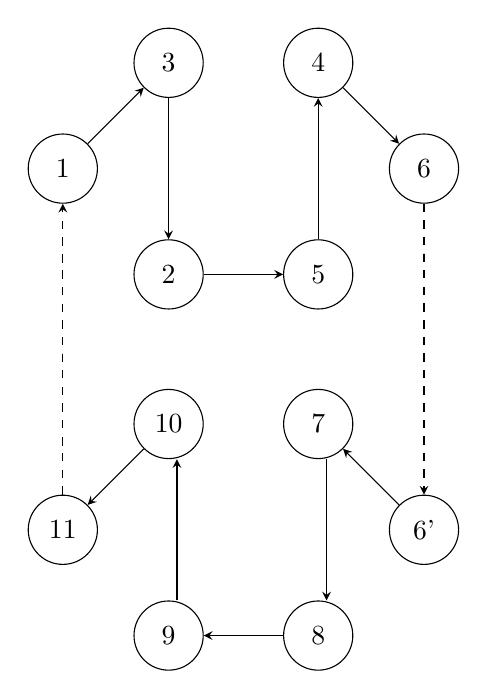
\begin{tikzpicture}[%
>=stealth,
node distance=1.9cm,
on grid,
auto
]
\node[state] (1){1};
\node[state] (3) [above right of=1]{3};
\node[state] (2) [below right of=1]{2};
\node[state] (4) [right of=3]{4};
\node[state] (5) [right of=2]{5};
\node[state] (6) [above right of=5] {6};
\node[state] (7) [below of=5] {7};
\node[state] (6') [below right of=7] {6'};
\node[state] (10) [left of=7] {10};
\node[state] (11) [below left of=10] {11};
\node[state] (9) [below right of=11] {9};
\node[state] (8) [right of=9] {8};

% solid: parent 1
\path[->] (11) edge [dashed, bend left=0] node  {} (1);
\path[->] (6) edge [dashed, bend left=0] node  {} (6');

\path[->] (6') edge [] node {}
         (7);
\path[->] ([xshift=0.7ex] 7.south) edge [] node {}
         ([xshift=0.7ex] 8.north);
\path[->] (8) edge [] node {}
         (9);
\path[->] ([xshift=0.7ex] 9.north) edge [] node {}
         ([xshift=0.7ex] 10.south);
\path[->] (10) edge [] node {}
         (11);
\path[->] (1) edge [bend left=0] node  {} (3);
\path[->] (3) edge [bend left=0] node  {} (2);
\path[->] (2) edge [bend left=0] node  {} (5);
\path[->] (5) edge [bend left=0] node  {} (4);
\path[->] (4) edge [bend left=0] node  {} (6);
\end{tikzpicture}
}
  \caption[Finaler Offspring $G_o$ erzeugt aus $G_1$ und $G_2$]{Der
  finale Zustand des Kindes $G_o$ nach Einfügen der Kantenmenge $E_c$
  und der kürzesten Teilwege der Komponenten. Gestrichelte Linien: Menge
  $E_c$, normale Linien: kürzeste Teilwege}
\end{figure}
%%\parbox[b][3cm][t]{4cm}{
%  \begin{tabular}{l r}
%    Komponente: & ${G_{c_1}}$ \\
%    Eingangsknoten: & $\{1\}$ \\
%    Ausgangsknoten: & $\{6\}$ \\
%  \end{tabular}
%}

\chapter{Lokale Suche mit 3-opt}
\section{Einleitung}
\section{Funktionsweise}
\section{Ergebnisse}

\chapter{Evolutionärer Algorithmus}
\section{Einleitung}
Ein „evolutionärer Algorithmus“ (kurz EA)
versucht ein Optimierungsproblem mithilfe der in der Biologie 
vorkommenden Gesetze der Evolution zu lösen. Ziel des Algorithmus ist
es ein Ergebnis über mehrere Generationen zu verbessern. Für das Traveling-
Salesman-Problem bedeutet dies, dass versucht wird, aus einer Menge
von zufällig generierten Rundreisen, eine möglichst kurze Rundreise zu
finden. In diesem Kapitel wird beschrieben, welcher EA bei der
Implementierung verwendet wurde.

\section{Basis}

\begin{figure}[H]
\begin{tikzpicture}[scale=1,align=center]
  \def \r {\textwidth/3}
  \def \margin {4}
  \node (rekombination) at (0:\r) {Rekombination};
  \node (paarungsselektion) at (60:\r) {Paarungs-\\selektion};
  \node (terminierungsbedingung) at (120:\r) {Abbruch-\\bedingung};
  \node (umweltselektion) at (180:\r) {Umwelt-\\selektion};
  \node (bewertung) at (240:\r) {Bewertung};
  \node (mutation) at (300:\r) {Mutation};

  \node (init) at (145:\r *1.75) {Init};
  \path[draw, ->, >=latex] (init) .. controls (165:\r *1.75) and (165:\r) ..
                  (terminierungsbedingung.south west);

  \draw[<-, >=latex] (4:\r) arc (4:50:\r);
  \draw[<-, >=latex] (305:\r) arc (305:356:\r);
  \draw[<-, >=latex] (246:\r) arc (246:292:\r);
  \draw[<-, >=latex] (186:\r) arc (186:235:\r);
  \draw[<-, >=latex] (130:\r) arc (130:175:\r);
  \draw[<-, >=latex] (75:\r) arc (75:100:\r);

  %% this goes form node to node in y cycle but because of the points
  %% where it leaves each node it makes the image loook wonky
  %
  % \path[draw] (rekombination) .. controls (20:5cm) and (40:5cm) ..
  % (paarungsselektion) .. controls (80:5cm) and (100:5cm) ..
  % (terminierungsbedienung) .. controls (140:5cm) and (160:5cm) ..
  % (umweltselektion) .. controls (200:5cm) and (220:5cm) ..
  % (bewertung) .. controls (260:5cm) and (280:5cm) ..
  % (mutation) .. controls (320:5cm) and (340:5cm) ..
  % (rekombination);

\end{tikzpicture}
\caption[Standardablauf eines evolutionären Algorithmus]{Der
  Standardablauf eines evolutionären Ablaufs}
\end{figure}
Der EA, der in diesem Projekt verwendet wurde, basiert auf einer
Arbeit von Yuichi Nagata und David Soler und weicht an manchen
Stellen vom dargestellten Standard ab~\cite{nagata}. Die entsprechenden
Parameter des EA sind in der Ausarbeitung zu GAPX von Tinós et al.
enthalten~\cite{gapx}.

\begin{algorithm}[H]
\caption{EA nach Nagata und Soler }\label{alg:ea}
\begin{algorithmic}[1]
  \Procedure{$EA$}{$GenLimit$}
    \State $P \gets pop\_init()$\Comment{Initiale Generation}
    \While{Abbruchbedingung nicht erfüllt}
      \State $(G_1, G_2) \ gets selection(P)$
      \State $G_o \gets crossover(G_1, G_2)$
      \If{Crossover hat Lösung nicht verbessert}
        \State $G_o \gets mutation(G_o)$
      \EndIf
      \State $P \gets append(P, G_o)$
      \If{Beste Lösung nach 20. Gen nicht verbessert}
        \State Nachbarschaftsgröße für ls3opt erhöhen
        \State $P = immigration(P)$\Comment{siehe Bem. 10}
      \EndIf
      \State $P = next\_generation(P)$
    \EndWhile
    \State \textbf{return} $best\_solution$
  \EndProcedure
\end{algorithmic}
\end{algorithm}
\begin{bem}
  Bei der Immigration werden alle Rundreisen, bis auf die Beste, durch
  neue zufällig generierte Rundreisen ersetzt, die mit „ls3opt“
  verbessert werden. Diese Funktion ist nicht
  Teil unserer Implementierung. Wir haben uns gegen die Immigration
  entschieden, da die Laufzeit von „ls3opt“ bereits sehr hoch ist und 
  durch „ls2opt“ (siehe Abschnitt Mutation) auch zufällige neue Rundreisen 
  entstehen.
\end{bem}
\section{Initialisierung}
In der Initialisierungsphase des EA werden $n$ Rundreisen aus einem
vollständigen Graphen zunächst zufällig erzeugt. Direkt im Anschluss
wird das in \hyperref[alg:ls3opt_run]{Algorithmus 5} vorgestellte Verfahren 
„ls3opt“ angewendet, um die
Rundreise an lokalen Stellen zu verbessern. Die initiale
\textit{Nachbarschaftsgröße für „ls3opt“ beträgt 10}. Sie wird um 1
inkrementiert, falls in den letzten 20 Generationen die beste Lösung
nicht verbessert wurde.
\section{Abbruchbedingung}
Der EA wird beendet, wenn \textit{1500 Generationen} durchlaufen wurden, oder
die bekannte optimale Lösung erreicht wurde. 
\section{Paarungsselektion}
Zur Selektion einer Rundreise wird eine \textit{Turnierselektion} angewendet, 
bei der zwei zufällige Rundreisen ausgewählt werden~\cite{weicker}. Jene mit dem
besseren Fitness-Wert wird mit einer \textit{Wahrscheinlichkeit von 0,8} als 
Elternteil verwendet~\cite{gapx}. Die Selektion findet also zwei mal 
(für $G_1$ und für $G_2$) statt. Sind die beiden Elternteile $G_1$ und
$G_2$ bestimmt, kann die Rekombination mittels GAPX durchgeführt werden.
\section{Rekombination}
Als Rekombinationsoperator wurde GAPX verwendet, welcher in
\hyperref[gapx_einleitung]{Kapitel 2}
ausführlich beschrieben wurde. Zwei Rundreisen müssen vorher mithilfe
der Paarungsselektion ausgewählt
werden. Anschließend kann der Crossover, wie in
\hyperref[alg:crossover_ea]{Algorithmus 1}
beschrieben, angewandt werden.
\section{Mutation}
Die Mutation wird bei allen Rundreisen durchgeführt, die einen
schlechteren Fitness-Wert haben als die derzeit beste Rundreise. 
Bei der Mutation wird eine zufällige Anzahl von „ls2opt“-Vorgänge
(Anzahl $\leq 10$) durchgeführt. Nach der Modifikation der Rundreise wird
zusätzlich noch ein „ls3opt“-Vorgang, wie in \hyperref[alg:ls3opt_run]{Algorithmus 5} 
erläutert, durchgeführt.

\begin{bem}
Bei einem „ls2opt“-Vorgang werden an zufälligen zwei zufälligen Stellen
zwei Kanten gelöscht und in einer anderen Art wieder verbunden. Bei
diesem Vorgang kann der Fitness-Wert der Rundreise schlechter werden.
Mit „ls2opt“ wird versucht eine höhere Vielfalt in der Population zu
erreichen.
\end{bem}

\section{Bewertung}
Die Rundreise wird mittels einer Fitness-Funktion $f$ bewertet.
Zur Ermittlung der Kantengewichte in einem Grpahen $G = (V, E)$ wird
eine Funktion $d(e)$, mit $e \in E$ definiert, die für eine Kante das
entsprechende Gewicht zurückgibt.
\begin{align*}
   f(G) = \sum_{e \in E} d(e)
\end{align*}
Die Summe der Kantengewichte entspricht der Fitness des Graphen von
$G$. Um so kleiner der Wert von $f(G)$, um so besser ist die Fitness des
Graphen.

\section{Umweltselektion}
\textit{Elitismus} wird angewandt,
um die beste Rundreise immer in die nächsten Generation zu übernehmen.
Der Fitness-Wert der besten Rundreise kann sich während des
evolutionären Algorithmus somit niemals verschlechtern. Die beste Lösung wird
zurückgegeben, wenn die Abbruchbedingung erreicht wurde.
\section{Parameterübersicht}
\begin{tabular}{l|p{5.4cm}}
  \textbf{Parameter} & \textbf{Wert} \\
  \hline
  Maximum Generationen & 1500 \\
  \hline
  Nachbarschaftsgröße „ls3opt“ & 10 \\
  \hline
  Erhöhung Nachbarschaftsgröße „ls3opt“ & 1 \\
  \hline
  Paarungsselektion & Turnierselektion, \newline mit Wahrscheinlichkeit 0.8 \\
  \hline
  Rekombination & GAPX\\
  \hline
  Mutation & ls3opt, ls2opt\\
  \hline
  Umweltselektion & Elitismus \\
  \hline
\end{tabular}

% \input{./tex/conclusions.tex}
\chapter{Erlang}
Da wir den Algorithmus durch „message passing“ parallelisieren wollten
haben wir uns für Erlang als unsere Programmiersprache verwendet.  Die
Sprache wurde im „Ericsson Computer Science Laboratory“ entwickelt um
vor allem Telekommunikationsanwendungen zu entwickeln, wo viel Wert
auf Nachrichtenaustausch und Distribution gelegt wird.

Erlang ist eine funktionale Programmiersprache, obwohl einzelne
Prinzipien gebrochen werden, wenn praktische Probleme dies gebieten.
Zum Beispiel wird referenzielle Transparenz – „Ein Ausdruck kann mit
seinem Ergebnis ersetzt werden, ohne die Korrektheit des Programms zu
ändern“ – in Einzelfällen gebrochen, damit das Ergebnis von
\lstinline!now()! überhaupt sinnvoll sein kann.

Da Erlangs Prozesse initial deutlich weniger Speicher benötigen, sind
sie deutlich leichter als ein Systemprozess.  Die Nebenläufigkeit wird
in Erlang mittels threads realisiert, deren Scheduling von der Erlang
Runtime selber betrieben wird.  Der Unterschied zu vielen anderen
Sprachen ist dabei, dass das Scheduling „preemptive“ ist, dem
rechnenden Prozess also der Kern entzogen werden kann.

Ein Erlang Prozess entspricht ungefähr einer Node.  Diese kann nach
einmaliger Verbindung mit anderen Nodes kommunizieren, was ebenfalls
mit Erlangs „message passing“ funktioniert.  Für mehr Details dazu
siehe \cite[Kapitel~„Distribunomicon“]{lyse}.

\section{Vorteile}
Erlang hat sich hervorragend geeignet, das Programm nebenläufig zu
machen.  Deshalb fiel unsere Wahl überhaupt erst auf die Sprache.

Das Versenden und Empfangen von Nachrichten ist extrem einfach durch
das „pattern matching“ von Erlang.  In dem Modul \lstinline!digraph!
werden Graphen als Tupel \lstinline!{digraph, V, E, N, true}!
dargestellt.  \lstinline!V!, \lstinline!E! und \lstinline!N! werden
intern als Datenbanktabellen gehalten, auf die jeder Prozess in einer
Node zugreifen kann, weshalb nur die Referenz auf die Tabellen
versendet werden muss.

Auch kann man durch Nachrichten ein Interface für den Benutzer
erstellen, in dem man an dem Hauptprozess eine Nachricht schickt und
er darauf antwortet.  Darüber hinaus gibt es Profiler wie
\lstinline!eprof!, welche einem die Flaschenhälse aufzeigen, an denen
man noch Optimierungen vornehmen kann.

\section{Nachteile}
\label{sec:disadv}
Für rechenintensive Aufgaben ist Erlang ungeeignet.  Dynamische
Sprachen haben generell das Problem, dass sie Typinformationen zur
Laufzeit haben müssen und der Kompiler deshalb weniger Optimierungen
vornehmen kann.  Es führt außerdem dazu, dass der Typ zur Laufzeit
überprüft werden muss, was ebenfalls Rechenzeit kostet.

Generell wird davon abgeraten, die Sprache für solche Zwecke zu
benutzen, da Erlang dafür nicht konzipiert wurde
\cite[Kapitel~3]{lyse}.

\subsection{\gtwght}
\label{subsec:get-weight}

Die Funktion \gtwght\ hat uns das Gewicht zwischen zwei Knoten in dem
Graphen zurückgegeben.  Als wir unseren Profiler benutzt haben,
stellte sich heraus, dass über 90\% der Aufrufe, und damit auch ein
Großteil der Zeit, dieser Funktion zufallen.  Deshalb hatten wir
versucht \gtwght\ zu optimieren, da die Anzahl der Aufrufe nicht
reduzieren werden konnte.

Zu erst wurde die Funktion so geschrieben, dass \gtwght\ den Graphen
selbst übergeben bekommt und dann auf dessen Tabellen eine
Datenbankabfrage macht.  Obwohl die In-Memory-Datenbank, in Erlang
wird diese ets genannt, einen konstanten Zeitaufwand für Lese- und
Schreiboperationen hat, war die konstante Zeit zu hoch.  Deshalb haben
wir vorher eine Liste mit allen Kanten erstellt aus denen wir mit
Hilfe von „pattern matching“ direkt den gefundenen Wert zurückgeben
konnten.  Das hatte uns eine durchschnittliche Zeit von 0,13 Sekunden
pro Aufruf erbracht.

Da immer noch die Laufzeit von \gtwght\ dominiert wurde, hatten wir
weiterhin versucht durch eine „Native Implemented Function“ (NIF) in C
die Zeit pro Aufruf zu reduzieren.  Das Resultat hat die Zeit pro
Aufruf leider verschlechtert, da die Makros für die Datenkonvertierung
(von Erlangs dynamischen Termen zu C-Typen) zu viel Zeit beansprucht.

Das war einer der Punkte, der im Nachhinein die Laufzeit drastisch
verschlechtert hat.  Es gibt in Erlang zwar auch Arrays, diese sind
allerdings funktional und bieten vor allem keinen wahlfreien
Speicherzugriff \cite[Kapitel~11]{lyse}.  Dieser Teil wäre in einer
Sprache wie C schnell und intuitiv gewesen, da einfach nur ein Zugriff
auf ein zweidimensionales Array an den übergebenen Indizes nötig
gewesen wäre.

\chapter{Parallelisierung}


\begin{SCfigure}
  \centering
  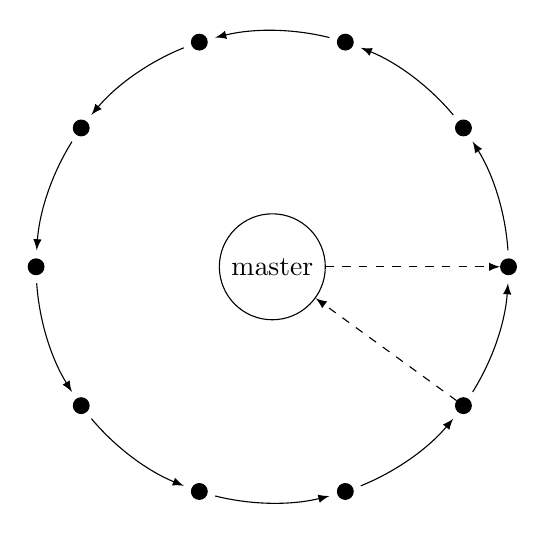
\begin{tikzpicture}
    [place/.style={circle,
      inner sep=0pt,minimum size=2mm}]
    %% from http://www.texample.net/tikz/examples/cycle/
    % Author : Jerome Tremblay
    \def \n {10}
    \def \radius {3cm}
    \def \margin {4} % margin in angles, depends on the radius

    \foreach \s in {1,...,\n}
    {
      \node[draw, circle, fill=black, place] (\s) at ({360/\n * (\s - 1)}:\radius) {};
      \draw[->, >=latex] ({360/\n * (\s - 1)+\margin}:\radius)
      arc ({360/\n * (\s - 1)+\margin}:{360/\n * (\s)-\margin}:\radius);
    }

    \node[draw, circle] (master) at (0:0) {master};
    \draw[->, >=latex, dashed] (master) -- (1);
    \draw[->, >=latex, dashed] (\n) -- (master);
  \end{tikzpicture}
  \caption{\label{fig:mult-subpop}Es werden mehrere Subpopulationen
    erzeugt, die dem jeweils nächsten Prozess dann Teile aus der
    eigenen Population zusenden.  }
\end{SCfigure}

\begin{SCfigure}
  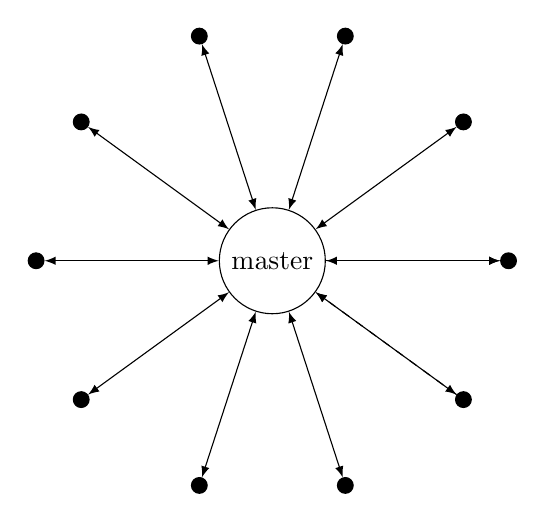
\begin{tikzpicture}
    [place/.style={circle,
      inner sep=0pt,minimum size=2mm}]
    \def \n {10}
    \def \radius {3cm}
    \def \margin {4} % margin in angles, depends on the radius

    \node[draw, circle] (master) at (0:0) {master};

    \foreach \s in {1,...,\n}
    {
      \node[draw, circle, fill=black, place] (\s) at ({360/\n * (\s - 1)}:\radius) {};
      \draw[<->, >=latex] (master) -- (\s);
    }

    \draw[->, >=latex, dashed] (master) -- (1);
    \draw[->, >=latex, dashed] (\n) -- (master);
  \end{tikzpicture}
  \caption{\label{fig:topology-central} Die
    Kindprozesse erzeugen einzelne Rundreisen und schicken diese an
    den „master“ zurück.  Dieser muss die Rundreisen dann in die
    eigene Population einsortieren.}
\end{SCfigure}

\chapter{Ergebnisse}
Unsere Ergebnisse wurden mit denen der Authoren verglichen.  Dabei
sind unsere Lösungen konsistent schlechter.

{
  \setmainfont[Numbers={Uppercase,Monospaced}]{Vollkorn}
  \begin{tabular}{lrrr}
    Problem & Beste Lösung & Erreichte Fitness & Generationen \\
    \hline
    br17    & 39           & 39                & 1            \\
    ftv33   & 1286         & 1296              & 199          \\
    ftv35   & 1473         & 1475              & 196          \\
    ftv38   & 1530         & 1536              & 286          \\
    ftv44   & 1613         & 1653              & 237          \\
    ftv47   & 1776         & 1794              & 233          \\
    ftv55   & 1608         & 1691              & 252          \\
    ry48p   & 14422        & 14608             & 313          \\
  \end{tabular}
}

\begin{figure}[ht]
    \centering
    \begin{subfigure}[b]{0.45\textwidth}
      \includegraphics[width=\textwidth]{../research/scores/ry48p-300-12}
      \caption{ry48p-300-12}
      \label{fig:ry48p-300-12}
    \end{subfigure}
    ~ %add desired spacing between images, e. g. ~, \quad, \qquad, \hfill etc.
      %(or a blank line to force the subfigure onto a new line)
    \begin{subfigure}[b]{0.45\textwidth}
      \includegraphics[width=\textwidth]{../research/scores/br17-300-24}
      \caption{br17-300-24}
      \label{fig:br17-300-24}
    \end{subfigure}

    % add desired spacing between images, e. g. ~, \quad, \qquad, \hfill etc.
    %(or a blank line to force the subfigure onto a new line)
    \begin{subfigure}[b]{0.45\textwidth}
      \includegraphics[width=\textwidth]{../research/scores/ftv33-300-12}
      \caption{ftv33-300-12}
      \label{fig:ftv33-300-12}
    \end{subfigure}
    ~
    \begin{subfigure}[b]{0.45\textwidth}
      \includegraphics[width=\textwidth]{../research/scores/ftv44-300-12}
      \caption{ftv44-300-12}
      \label{fig:ftv44-300-12}
    \end{subfigure}
    \caption{\label{fig:fitness-plots} Fitnesswerte über die ersten
      100 Generationen}
\end{figure}


\appendix




% Bibliography:
\clearpage
\addcontentsline{toc}{chapter}{Literatur}



\end{document}
